\section{Attenuation}

In this part of the lab course, we investigated the attenuation of radiation from $^{137}$Cs through copper.
The attenuation of radiation can be calculated with:
\begin{equation}
I(d) = I_0 e^{\frac{\mu}{\rho} d  }
\end {equation}
Where $I$ is the attenuated quantity, $I_0$ is this quantity without attenuatiuon, $\frac{\mu}{\rho}$ is the mass attenuation coeficient and $d$ is the lenght over which the attenuation takes place.
To measure these, we took the spectra of $^{137}$Cs, shielded through multiple layers of copper.
Natural occuring copper only has stable isotopes, which means that this shielding shouldn't give much extra background radiation
The measured spectra can be seen in Fig. \ref{attenuation_spectra}.
\begin{figure}[h]
\begin{subfigure}{.5\textwidth}
  \centering
  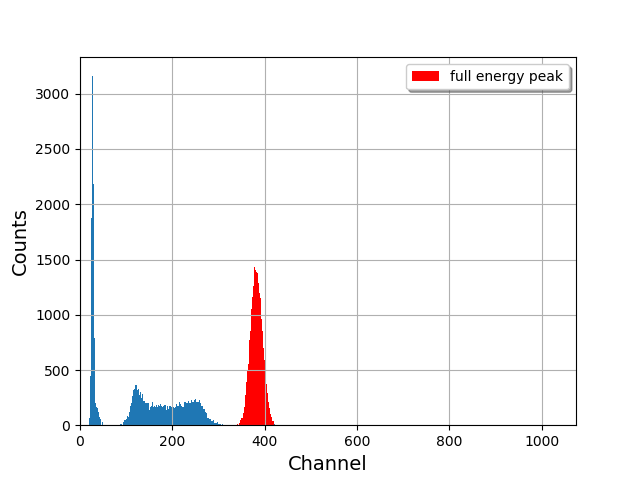
\includegraphics[width=.9\linewidth]{../Plots/attenuation_0.png}
  \caption{no copper}
\end{subfigure}%
\begin{subfigure}{.5\textwidth}
  \centering
  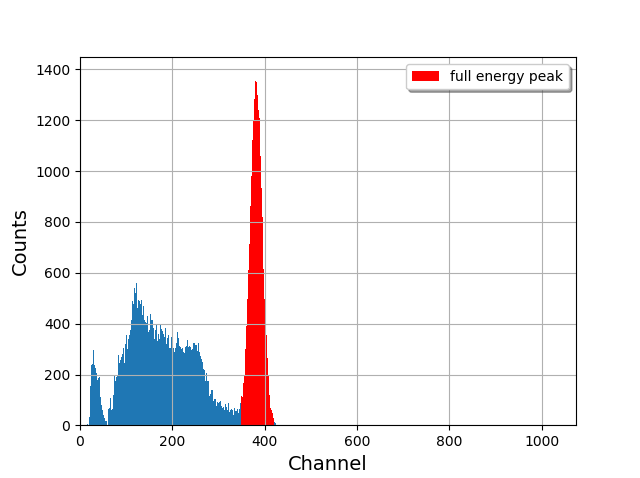
\includegraphics[width=.9\linewidth]{../Plots/attenuation_1.png}
  \caption{4 mm of copper}
\end{subfigure}%
 \vskip\baselineskip
\begin{subfigure}{.5\textwidth}
  \centering
  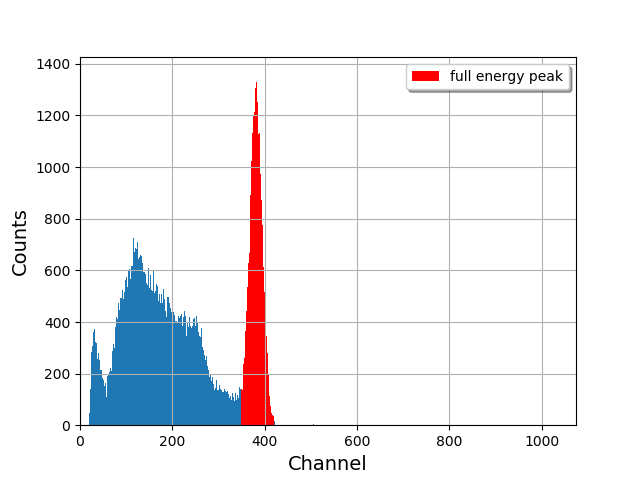
\includegraphics[width=.9\linewidth]{../Plots/attenuation_2.png}
  \caption{8 mm of copper}
\end{subfigure}%
\begin{subfigure}{.5\textwidth}
  \centering
  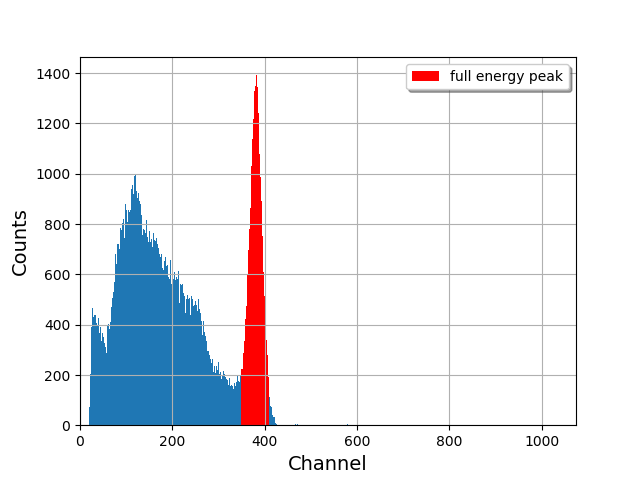
\includegraphics[width=.9\linewidth]{../Plots/attenuation_3.png}
  \caption{4 mm of copper}
\end{subfigure}%
 \vskip\baselineskip
\begin{subfigure}{.5\textwidth}
  \centering
  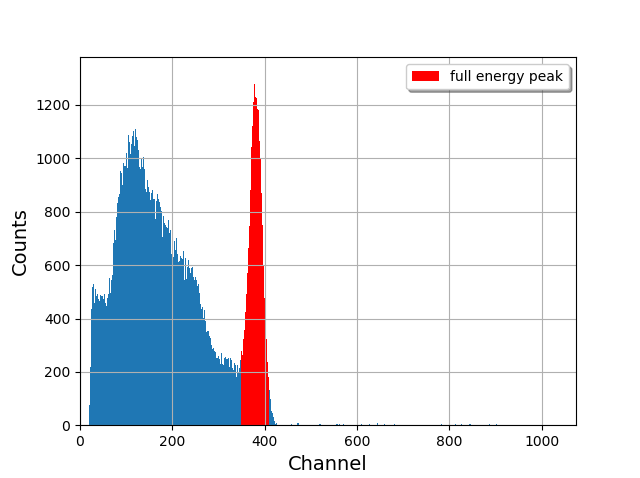
\includegraphics[width=.9\linewidth]{../Plots/attenuation_4.png}
  \caption{16 mm of copper}
\end{subfigure}%
\caption{Spectra of $^{137}$Cs with copper shielding}
\label{attenuation_spectra}
\end{figure}
Time for measurement was adjusted, that every peak has at least a maximum counting of 1000 events, to give us a better statistic.
Background radiation was again substracted from every spectrum.

We can see, that even the lowest shielding with 4 mm copper was enough to remove the beta-peak on the far left of the spectrum.
This can easily be explained with the low range of electrons in matter and was expected.
As attenuated quanitty, we used the full energy peak to calculate the counts per second from this peak.
This was calculated gain with Eq. \ref{gauss_area}.
The results can be seen in Table \ref{attenuation_values}.
\begin{table}[h]
\centering
\begin{tabular}{c |c }
\hline
Counts per second [s$^{-1}$] & thickness [mm] \\
\hline
334.1 & 0 \\
263.7 & 4 \\
208.6 & 8 \\
161.7 & 12 \\
127.1 & 16 \\
\hline
\end{tabular}
\caption{Attenuation through copper}
\label{attenuation_values}
\end{table}
Plotting this data enabled us to fit the values according to the function:
\begin{equation}
I(d) = I_0 e^{a \cdot d}
\end {equation}
With $a = \frac{\mu}{\rho}$.
Given the density of copper at $300$K ($8.96 \text{gcm}^{-3}$) made it possible to calculate the attenuation coefficient of copper from this fit-parameter.
The data and fit can be seen in Fig. \ref{attenuation_fit}
\begin{figure}[h]
  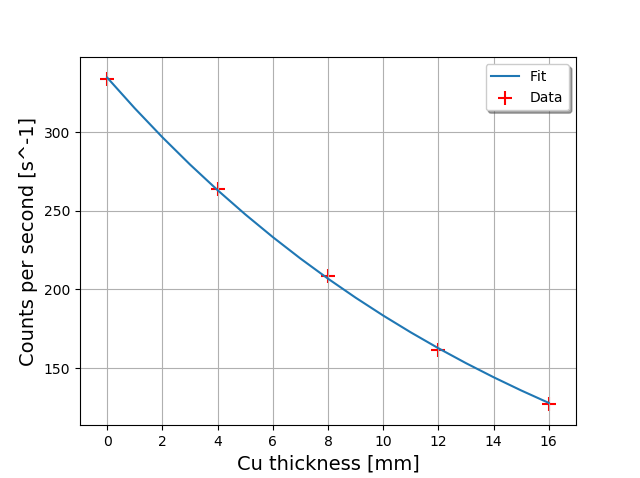
\includegraphics[width=\linewidth]{../Plots/attenuation.png}
  \caption{Data and fit of the attenuation}
  \label{attenuation_fit}
\end{figure}
We can directly see, that the data are well approximated through the exponential function.
The fit parameter $a$ was calculated to $a = (60.17 \pm 0.26)$.
We can now calculate the attenuation coefficient $(\mu = \frac{a}{\rho}$), which gives us:

$\mu = (6.715 \pm 0.029) \cdot 10^{-2}$ $\text{cm}^2 \text{g}^{-1}$

As a literature value for comparision, we got $\mu = 7.3 \cdot 10^{-2}\text{cm}^2 \text{g}^{-1}$ (Quelle xcom einfügen).
\clearpage
